%!TEX options = --shell-escape
%!TEX program = xelatex

\documentclass[11pt,a4paper]{dlove}

\title{\bfseries 基本无害的经济学 \LaTeX{} 技巧}
\author{\href{https://ddswhu.me/}{\bfseries 邓东升} \\  Elegant\LaTeX{} 项目组}
\date{\today}

\usepackage{xcolor}
\definecolor{firebrick}{rgb}{0.7, 0.13, 0.13}

\newcommand{\texmint}[1]{\mintinline{tex}{#1}}
\renewcommand{\emph}[1]{\textcolor{firebrick}{#1}}

\begin{document}


\maketitle

此文档为经济学专业的 \LaTeX{} 技巧总结,包括环境搭建、基础知识、参考文献以及幻灯片制作等内容,仅作为经济学专业的师生作为入门 \LaTeX{} 使用。使用 \texmint{dlove} \heart{} 模板和 \hologo{XeLaTeX} 编译完成。

\section{文档必读}
在写作文档时,我觉得有几个准则
\begin{itemize}
  \item 内容为王,不要过分追求格式,Word、Markdown、\LaTeX{} 无所谓;
  \item 导师为大,导师用什么,你用什么。
  \item 保持学习的态度,但是不要主次不分。
  \item 投稿用模板时,不要有自己的想法。具体来说,就是不管你对你所投稿的杂志给的官方模板有任何意见,请保留,不要尝试去改动里面的设置。你可能会问,你所用的模板和杂志的样稿不一样,不要紧张,投稿和发表本身模板就会不一样。
\end{itemize}

\section{环境搭建}
目前 \LaTeX{} 的主要发行版本如下:
\begin{itemize}
  \item \hologo{MiKTeX}:Windows 上的发行版,国内的 C\TeX{}\footnote{已过时,请尽量不要使用。} 使用的就是 \hologo{MiKTeX};
  \item \TeX{} Live:编辑器 \TeX{}works,跨系统,每年更新一个大版本,最新版为 TeX Live 2019;
  \item Mac\TeX{}:Mac 上的 \TeX{} Live,为了适应 Mac 系统做了一些细微的调整;
\end{itemize}

推荐使用 \TeX{} Live 2019,可以使用默认的 \TeX{}works 或者配合其他编辑器(比如 Sublime Text、Visual Studio Code)的插件进行编写,后面我们会细说这部分。

\subsection{安装 \TeX{} Live}
首先,我们进入 \TeX{} Live 的\href{https://www.tug.org/texlive/}{官网}地址,点击页面中的 \href{https://www.tug.org/texlive/acquire-netinstall.html}{download},然后可以选择在线安装或者下载安装文件之后离线安装,推荐使用离线安装。
\begin{itemize}
  \item \textbf{在线安装}:点击 \href{http://mirror.ctan.org/systems/texlive/tlnet/install-tl-windows.exe}{install-tl-windows.exe}(Windows) 或者 \href{http://mirror.ctan.org/systems/texlive/tlnet/install-tl-unx.tar.gz}{install-tl-unix.tar.gz}(Linux/Unix),视自己系统选择,然后按照提示进行安装。
  \item \textbf{离线安装}:首先下载镜像文件,点击 \href{https://ctan.org/mirrors}{generic mirror.ctan.org url},这个时候我们会跳转到 \TeX{} Live 的\href{https://ctan.org/mirrors}{镜像站},下拉找到国内的镜像站。在国内的镜像列表中,选择离自己比较近的地区的镜像进行下载\footnote{比如上海的用户可以选择\href{https://mirrors.sjtug.sjtu.edu.cn/ctan/}{上海交大的镜像地址},然后往上拉找到 \TeX{} Live,点击进入上海交大 \TeX{} Live 的\href{https://mirrors.sjtug.sjtu.edu.cn/ctan/systems/texlive/}{下载地址},选择 \href{https://mirrors.sjtug.sjtu.edu.cn/ctan/systems/texlive/Images/}{./images/},然后将 \href{https://mirrors.sjtug.sjtu.edu.cn/ctan/systems/texlive/Images/texlive.iso}{texlive.iso}下载即可。}。下载镜像文件之后,使用资源管理器或者镜像挂载工具\footnote{推荐使用 \href{http://wincdemu.sysprogs.org/}{WinCDEmu} 进行挂载,WinCDEmu 下载后直接安装即可,这里不再赘述。}进行挂载,\textsf{\textcolor{FireBrick}{请不要使用压缩软件对镜像文件解压缩}}。
\end{itemize}

更多的关于 \TeX{} Live 的安装问题,可以参考\href{https://github.com/OsbertWang}{啸行}的\href{https://github.com/OsbertWang/install-latex}{一份简短的关于 \LaTeX{} 安装的介绍}。

\subsection{配置编译环境}
在安装好 \TeX{} Live 之后,我们需要选择一个编辑器,目前主流的编辑器有:
\begin{itemize}
  \item \href{http://www.winedt.com/}{WinEdt},\TeX{} 专用,过去 Windows 上非常流行的编辑器,收费软件,编辑方便,有输入辅助面板,编码支持不好,适合新手,但不推荐;
  \item \href{http://texstudio.sourceforge.net/}{\TeX{}studio},\TeX{} 专用,开源软件,兼顾了易用性以及可定制性,代码提示优秀,有输入辅助面板,适合新手,推荐全阶段使用。
  \item \TeX{}works,\TeX{} 专用,\TeX{} Live 自带的编辑器,界面非常简洁,对于新手不友好,自动补全功能还可以,需要的可以参考我之前的一个总结:\href{https://github.com/EthanDeng/texworks-autocomplete}{\TeX{}works 自动补全功能},推荐不想安装额外软件的用户。
  \item \href{http://www.sublimetext.com/}{Sublime Text},颜值很高、高可定制化的文本编辑器,非 \TeX{} 专用,付费软件,界面非常简洁,自动补全功能完善,代码高亮非常优秀,支持自定义代码片段,插件开发成熟,极度不适合新手,另外插件安装可能受限,极度不适合无法科学上网的用户,只适合高玩以及颜值主义者。
  \item Visual Studio Code, 微软推出的高可定制化文本编辑器,非 \TeX{} 专用,免费软件。可配置快捷编译按钮,自动补全、代码高亮很优秀,插件体验良好,但由于处于不断更新迭代过程,中间可能会有重大改动,需要关注开发者。推荐熟悉 \LaTeX{} 的用户使用。
\end{itemize}

我在我的小圈子里做了一个 \LaTeX{} 编辑器体验调查,表~\ref{tab:editor} 列出了各个编辑器的用户平均评分,此表为主观打分,仅供参考。此表的绘制参考了~\cite{jake2019} 的 \TikZ{} 代码。如果你对这些编辑器有自己的评价,欢迎 \href{https://github.com/EthanDeng/mhlatex4econ/blob/master/archive/LaTeX 编辑器对比评分表.xlsx}{下载评分表},对自己熟悉的编辑器打分,然后发给我 \email{ddswhu@outlook.com},我将加入到这个评分表中。

\begin{table}[htbp]
  \centering
  \caption{\LaTeX{} 编辑器对比}
    \begin{tabular}{cccccc}
    \toprule
             &  WinEdt      &  \TeX{}studio  & \TeX{}works   &  Sublime Text &  VS Code     \\
             \cline{5-6}
    插件依赖  &        &   &  &  \href{https://latextools.readthedocs.io/en/latest/}{\LaTeX{}Tools} &  \href{https://marketplace.visualstudio.com/items?itemName=James-Yu.latex-workshop}{\LaTeX{} Workshop}   \\
    \midrule
    主流系统  &  Win          &  全平台        & Linux/Win     &  全平台        &  全平台       \\
    软件类型  &  商业软件      &  开源软件       & 开源软件       &  商业软件       &  商业软件     \\
    软件价格  &  \href{https://item.taobao.com/item.htm?id=551105790596}{219 元}       &  0             &  0            &  \href{https://www.sublimehq.com/store/text}{80 美元}        &  0           \\
    授权方式  &  终身/教育     &               &               &  终身/个人      &               \\
    % 附加信息  &  教育版本      &               &               &  三年更新       &               \\
    代码高亮  &  \stars{2.7}  &  \stars{3.2}  &  \stars{1.5}  &  \stars{4.3}  &  \stars{4.5}  \\
    颜色主题  &  \stars{2.3}  &  \stars{2.2}  &  \stars{1.0}  &  \stars{4.0}  &  \stars{4.0}  \\
    自动补全  &  \stars{2.7}  &  \stars{3.4}  &  \stars{2.0}  &  \stars{3.5}  &  \stars{4.0}  \\
    代码片段  &  \stars{2.7}  &  \stars{2.4}  &  \stars{0.5}  &  \stars{3.8}  &  \stars{4.0}  \\
    辅助输入  &  \stars{4.0}  &  \stars{3.4}  &  \stars{0.5}  &  \stars{2.3}  &  \stars{3.3}  \\
    开发完成  &  \stars{4.0}  &  \stars{3.8}  &  \stars{4.5}  &  \stars{3.5}  &  \stars{4.0}  \\
    推荐指数  &  \stars{2.7}  &  \stars{4.0}  &  \stars{1.5}  &  \stars{3.0}  &  \stars{4.3}  \\
    \bottomrule
    \end{tabular}%
  \label{tab:editor}%
\end{table}%


\section{基础知识}

\subsection{命令与环境}
\textbf{命令}和\textbf{环境}是 \LaTeX{} 最重要的组成部分,因此我们先了解下这两个概念。

命令由反斜杠 \mintinline{tex}{\} 引导,一般的形式为 \mintinline{tex}{\cmd[可选参数]{必选参数}},命令名全部由\textcolor{FireBrick}{英文字母}构成,并且大小写敏感,因此 \mintinline{tex}{\LaTeX{}} 是对的,而 \mintinline{tex}{\latex{}} 是错的。必选参数可能有 0 个或者多个,无参数的命令为 \mintinline{tex}{\cmd},多个参数的形式为 \mintinline{tex}{\cmd[可选参数]{参数 1}{参数 2}...{参数 N}}。下面是一个示例:

\begin{code}
  无参数命令:\LaTeX{} \vline
  单参数命令:\textbf{加粗} \textit{Italic Style}
  多参数命令:\rule{2cm}{0.4pt}
\end{code}
\begin{preview}
  无参数命令:\LaTeX{} \quad  \vline\\
  单参数命令:\textbf{加粗} \textit{Italic Style} \\
  多参数命令:\rule{2cm}{0.4pt}
\end{preview}

这里对部分命令解释一下,\mintinline{tex}{\vline} 不带参数时,会输出一条高度为行高的竖线(vertical line),而 \mintinline{tex}{\textbf} 和 \mintinline{tex}{\textit} 分别为字体\textbf{加粗}(\textbf{bold face})和斜体(\textit{italic})的命令。\mintinline{tex}{\hrule} 类似于 \mintinline{tex}{\vline},用于画一个长为 2 \si{cm},宽度为 0.4 \si{pt} 的水平线段(horizontal rule)。

环境相对于命令而言,是更加高层的命令组合,用于实现一系列功能、格式的定制化。一个环境(environment)的基本结构为

\begin{code}
  \begin{环境名}
    % 内容
  \end{环境名}
\end{code}
\begin{rcode}
  \begin{环境名}[可选参数]{必需参数}
    % 内容
  \end{环境名}
\end{rcode}

当没有\textit{可选参数}或者\textit{必需参数},可以直接将其对应的括号 \mintinline{tex}{[]} 以及 \mintinline{tex}{{}} 去掉。下面以 \LaTeX{} 中默认的环境来举例说明环境的用法。如果我们需要对一段文字进行居中,则可以使用 \mintinline{tex}{center} 环境\footnote{居左为 \mintinline{tex}{flushleft} 环境,居右为 \mintinline{tex}{flushright} 环境。}。

\begin{code}
  \begin{center}
    落霞与孤鹜齐飞,秋水共长天一色。渔舟唱晚,响穷彭蠡之滨;雁阵惊寒,声断衡阳之浦。
  \end{center}
\end{code}
\begin{preview}
  \begin{center}
    落霞与孤鹜齐飞,秋水共长天一色。渔舟唱晚,响穷彭蠡之滨;雁阵惊寒,声断衡阳之浦。
  \end{center}
\end{preview}

关于带参数的环境的使用,后文有很多例子,这里不赘述。另外,你可能会问 \LaTeX{} 内置哪些环境可以使用,以及他们分别用来干嘛的,关于这部分内容,你可以参考~\cite{latexenvironments} 的 \href{http://www.personal.ceu.hu/tex/environ.htm}{\LaTeX{} Standard Environments}。

载入 \mintinline{tex}{enumerate} 宏包之后,\textbf{列表}环境可以传入参数改变标签:

\begin{code}
  \begin{itemize}
    \item First item;
    \item Second item;
    \item Third item。
  \end{itemize}
\end{code}
\begin{preview}
  \begin{itemize}
    \item First item;
    \item Second item;
    \item Third item。
  \end{itemize}
\end{preview}

\subsection{最简示例}
\begin{code}
\documentclass{article}
% 导言区
\begin{document}
Hello World.
\end{document}
\end{code}
\begin{preview}
Hello World.
\end{preview}

其中,\texmint{\documentclass} 是文档类型\textbf{命令},声明本文档是文章(article),而正文部分需要放在 \texmint{\begin{document}} 和 \texmint{\end{document}} 之间,比如上面例子中的 \texmint{Hello World} 就是正文内容。

而在 \texmint{\documentclass} 和 \texmint{\begin{document}} 之间的部分,我们称为\textbf{导言区}。在这部分,我们可以引入功能宏包,进行选项设置或者定义一些命令等等。\LaTeX{} 本身能做很多事情,但是很多定制化的功能或者需求需要宏包支持,因此几乎全部的文档都是基于 \LaTeX{} 基本文档类型的命令和环境配合其他宏包命令、环境共同使用的。

\subsection{文档类型}

\LaTeX{} 默认的文档类型(简称\textbf{文类})主要有
\begin{itemize}
  \item 文章文类:\texmint{article};
  \item 书籍文类:\texmint{book};
  \item 演示文稿:\texmint{beamer};
  \item 报告文类:\texmint{report};
\end{itemize}

声明文类时可以设置文类选项,多个文类选项用英文逗号隔开,命令为 \mintinline{tex}{\documentclass[文类选项 1, 文类选项 2, ...]{文类}}。

以文类 \texmint{article} 为例,由于 \texmint{article} 的默认纸张为 legal 大小,将其更改为 A4 纸张,需要使用 \mintinline{tex}{\documentclass[a4paper]{article}}。我们也可以通过文类选项设置字体大小,比如正文字体大小为 11pt 的设置为 \mintinline{tex}{\documentclass[a4paper,11pt]{article}}。文类选项有:
\begin{itemize}
  \item \textsf{字体大小} (\texmint{10pt}, \texmint{11pt}, \texmint{12pt})
  \item \textsf{纸张大小} (\texmint{a4paper}, \texmint{letterpaper}, etc.)
  \item \textsf{章节开启方式} (\texmint{openright}, \texmint{openany})
  \item 草稿模式 (\texmint{draft})
  \item 多栏模式 (\texmint{onecolumn}, \texmint{twocolumn})
  \item 公式格式 (\texmint{fleqn} and \texmint{leqno})
  \item 横向打印 (\texmint{landscape})
  \item 边距选项 (\texmint{oneside}, \texmint{twoside})
  \item 封面选项 (\texmint{notitlepage}, \texmint{titlepage})
\end{itemize}

其中前三组选项为常用文类选项,如果想了解更多文类选项的内容,也可以参考~\href{https://texblog.org/2013/02/13/latex-documentclass-options-illustrated/}{\LaTeX{} Documentclass Options Illustrated}。

\textbf{GitHub Issue}: \href{https://github.com/EthanDeng/mhlatex4econ/issues/6}{怎么设置字号}。

\subsection{添加并修改目录}
这是 GitHub 上的一个 issue,原文 \href{https://github.com/EthanDeng/mhlatex4econ/issues/7}{如何加目录?}
\subsubsection{目录命令}
首先,在 \LaTeX{} 中添加目录的方法如下:将 \mintinline{tex}{\tableofcontents} 放在你所需要目录出现的地方,一般来说,我们会把目录放在封面信息之后,也就是 \mintinline{tex}{\maketitle} 之后。

\textsf{需要注意的时候,在涉及到超链接、目录、参考文献的时候,都需要编译至少 2 遍才能得到正确的目录、超链接以及参考文献引用。}

\subsubsection{额外添加信息}
在知道如何添加目录之后,如果想把某一章或者某一节(无编号)也添加到目录中,那么可以使用 \texmint{addcontentsline} 命令。具体用法

\begin{code}
  \chapter*{Acknowledgements}
  \addcontentsline{toc}{chapter}{Acknowledgements}
\end{code}

第一行命令 \mintinline{tex}{\chapter*} 表示当前章节不编号,并且不放在目录中,章节名为 Acknowledgements;第二行命令表示在目录中添加一个章目录,名为 Acknowledgements(可以与之前的不一样,比如写成 Acknow.)的命令。

\subsection{宏包}

\begin{table}[htbp]
  \centering
  \caption{一些常见的功能宏包}
    \begin{tabular}{cccccc}
    \toprule
    \textbf{数学公式}  & \textbf{插图插表}   & \textbf{页面元素}   & \textbf{字体设置}   & \textbf{参考文献}  & \textbf{表格}        \\
    \midrule
    \texmint{amsmath} & \texmint{graphicx} & \texmint{geometry} & \texmint{fontspec} & \texmint{natbib}  & \texmint{booktabs}  \\
    \texmint{amsthm}  & \texmint{caption}  & \texmint{hyperref} & \texmint{ctex}     & \texmint{gbt7714} & \texmint{longtable} \\
    \texmint{amssymb} & \texmint{subfig}   &                    & \texmint{xeCJK}    &                   & \texmint{multirow}  \\
    \bottomrule
    \end{tabular}%
  \label{tab:pkg}%
\end{table}%

Question: \href{https://github.com/EthanDeng/mhlatex/issues/21}{如何查找自己需要的各种宏包?比如用于化学结构式,反应式?}

Answer:两种方法,
\begin{enumerate*}
  \item 直接在 \href{http://ctan.org/pkg}{CTAN} 搜索。\TeX{} Live 中自带的包有很多,你可以用关键字搜索,比如搜索 \textsf{chemical formula} 之类的词,然后去查看每个包的功能介绍,找到自己合适的包;
  \item 通过搜索引擎搜索。你可以在搜索引擎搜索 \textsf{latex chemical formula},特别关注 \href{https://tex.stackexchange.com/}{TeX - LaTeX Stack Exchange} 上的答案。
\end{enumerate*}

\begin{center}
  \begin{minipage}[c]{0.49\textwidth}
    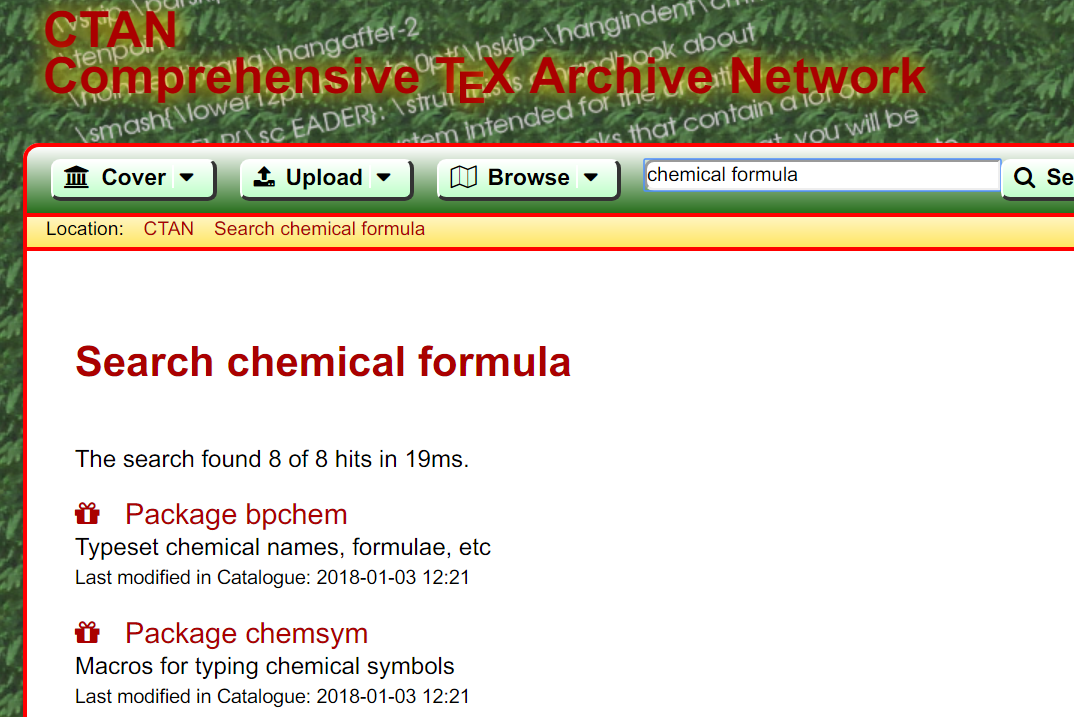
\includegraphics[width=\textwidth]{pkg-search-ctan.png}
  \end{minipage}
  \begin{minipage}[c]{0.49\textwidth}
    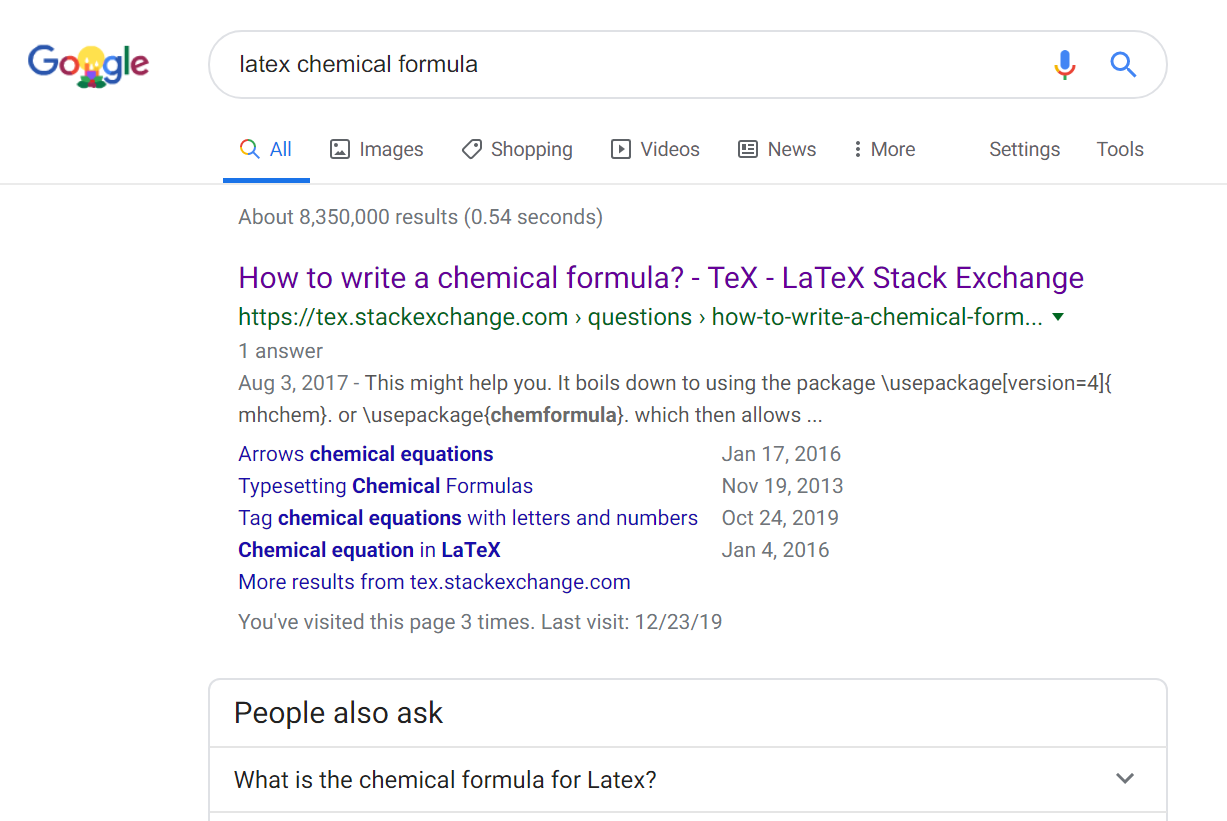
\includegraphics[width=\textwidth]{pkg-search-google.png}
  \end{minipage}  
\end{center}


备注:如果本地已经安装 \TeX{} Live,可以通过命令提示符(\textsf{command line/cmd} 或者 \textsf{terminal})查看宏包说明文档,请注意这是每个宏包官方的、也是最好、最全面的文档,如果你不理解一些宏包选项或者设置,你可以通过此方法获取宏包官方文档。具体的,如果你想查找中文支持宏包 \mintinline{shell}{ctex} 的官方文档,可以在 cmd 里面输入 \mintinline{shell}{texdoc ctex},如图~\ref{fig:texdoc} 所示。

\begin{figure}
  \centering
  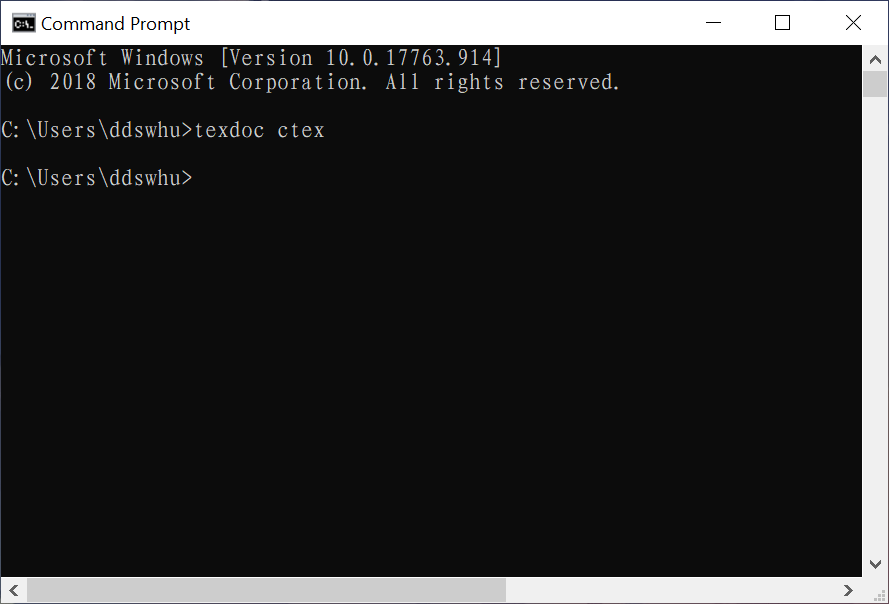
\includegraphics[width=0.5\textwidth]{image/texdoc.png}
  \caption{使用 \mintinline{shell}{texdoc} 命令查看 \TeX{} Live 本地的宏包说明文档\label{fig:texdoc}}
\end{figure}

\subsection{中文支持}

目前流行的中文支持有两个方式:
\begin{itemize}
\item \texmint{ctex} 宏包,或者与其相适应的 \texmint{ctexart} 等文类。
\item \texmint{xeCJK} 宏包,需要使用 \hologo{XeLaTeX} 编译。
\end{itemize}

\subsection{数学字母}
常用的一些希腊字母见表~\ref{tab:greek_letters},需要注意的是这些希腊字母需要在数学模式(比如 \texmint{$\alpha$})或者数学环境中使用。
\begin{table}[htbp]
  \centering
  \small
  \caption{希腊字母表}
    \begin{tabular}{llllll}
    \toprule
    \textsf{符号} & \textsf{命令} & \textsf{符号} & \textsf{命令} & \textsf{符号} & \textsf{命令} \\
    \midrule
    $\alpha$ & \texmint{\alpha} & $\iota$ & \texmint{\iota} & $\sigma$\; $\Sigma$ & \texmint{\sigma \Sigma} \\
    $\beta$ & \texmint{\beta} & $\kappa$ & \texmint{\kappa} & $\tau$ & \texmint{\tau} \\
    $\gamma$\; $\Gamma$ & \texmint{\gamma \Gamma} & $\lambda$ \; $\Lambda$ & \texmint{\lambda \Lambda} & $\upsilon$\; $\Upsilon$ & \texmint{\upsilon \Upsilon} \\
    $\delta$ \; $\Delta$ & \texmint{\delta \Delta} & $\mu$ & \texmint{\mu} & $\phi$\; $\Phi$ & \texmint{\phi \Phi} \\
    $\epsilon$ & \texmint{\epsilon} & $\nu$ & \texmint{\nu} & $\chi$ & \texmint{\chi} \\
    $\zeta$ & \texmint{\zeta} &  $\pi$ \; $\Pi$& \texmint{\pi \Pi} & $\psi$\; $\Psi$ & \texmint{\psi \Psi} \\
    $\eta$ & \texmint{\eta} & $\rho$ & \texmint{\rho}  & $\omega$\; $\Omega$ & \texmint{\omega \Omega} \\
    $\theta$ & \texmint{\theta} & $\varepsilon$ &  \texmint{\varepsilon} &       &  \\
    \bottomrule
    \end{tabular}%
  \label{tab:greek_letters}%
\end{table}%

\subsection{文本模式与数学模式}
在 \LaTeX{} 中,文本和数学是作为两个独立的不同模式存在的,如果需要在文本模式中输入数学式,需要使用英文状态下的美元符号 \mintinline{tex}{$} 将数学命令包围,比如 \texmint{$\alpha$} 输出为 $\alpha$。

\begin{code}
假设 $y_{i}$ 是被解释变量的第 $i$ 次观测,$x_{i}$ 是解释变量的第 $i$ 次观测,设定回归方程为 $y_{i} = \alpha + \beta x_{i} + \varepsilon_{i}$。
\end{code}
\begin{preview}
假设 $y_{i}$ 是被解释变量的第 $i$ 次观测,$x_{i}$ 是解释变量的第 $i$ 次观测,设定回归方程为 $y_{i} = \alpha + \beta x_{i} + \varepsilon_{i}$。
\end{preview}

\subsection{数学环境}
数学环境中,最简单的就是 \texmint{equation} 环境,这个环境会对数学公式进行自动编号,如果不需要编号,可以使用 \texmint{equation*} 环境。\par

\begin{code}
\begin{equation}
y_{i} = \alpha + \beta x_{i} + \varepsilon_{i}
\end{equation}
\end{code}
\begin{preview}
\begin{equation}
y_{i} = \alpha + \beta x_{i} + \varepsilon_{i}
\end{equation}
\end{preview}

\section{表格输入}
\LaTeX{} 中表格的输入并不太方便,最简单的一个表格示例如下:

\begin{code}
\begin{tabular}{ccc}
  English &  Context &   996   \\
  Right   &   Here   &  1024   \\
  Chinese & $\alpha$ & $\beta$ \\
\end{tabular}
\end{code}
\begin{preview}
\begin{center}
\begin{tabular}{ccc}
  English &  Context &   996   \\
   Right  &   Here   &  1024   \\
  Chinese & $\alpha$ & $\beta$ \\
\end{tabular}
\end{center}
\end{preview}

在上述命令中,创建表格的环境名为 \texmint{tabular},而 \texmint{tabular} 后的选项为列的对齐方式,分别有居中对齐(c),左对齐(l),右对齐(r),而同一行的不同列之间用 \& 隔开,而换行使用 \texmint{\\}。很显然,这种表格并不是我们想要的,我们需要加入一些表格框线:

\begin{code}
\begin{tabular}{|l|c|r|}
  \hline
  English &  Context &     996 \\
  Right   &   Here   &    1024 \\
  Chinese & $\alpha$ & $\beta$ \\
  \hline
\end{tabular}
\end{code}
\begin{preview}
\begin{center}
\begin{tabular}{|l|c|r|}
  \hline
  English &  Context &     996 \\
  Right   &   Here   &    1024 \\
  Chinese & $\alpha$ & $\beta$ \\
  \hline
\end{tabular}
\end{center}
\end{preview}

可以发现,\texmint{|} 为表格的列添加竖线,而 \texmint{\hline} 为表格的行添加了横线。

\subsection{三线表}

在实际写作中,我非常推荐大家使用三线表,而不要添加过多的横线或者竖线,利用 \texmint{booktabs} 宏包中的 \texmint{\toprule}、\texmint{\midrule} 以及 \texmint{\bottomrule} 能够非常方便的制作出三线表。示例如下:

\begin{code}
\begin{tabular}{lcr}
  \toprule
  Language &   Infor  &  Number \\
  \midrule
  English  &  Context &     996 \\
  Right    &   Here   &    1024 \\
  Chinese  & $\alpha$ & $\beta$ \\
  \bottomrule
\end{tabular}
\end{code}
\begin{preview}
\begin{center}
\begin{tabular}{lcr}
  \toprule
  Language &   Infor  &  Number \\
  \midrule
  English  &  Context &     996 \\
  Right    &   Here   &    1024 \\
  Chinese  & $\alpha$ & $\beta$ \\
  \bottomrule
\end{tabular}
\end{center}
\end{preview}

\subsection{长表格}
如果表格非常长,可以使用 \texmint{longtable} 代替 \texmint{table}。

\begin{code}
\begin{table}
  \begin{tabular}
    % 表格内容
  \end{tabular}
\end{table}
\end{code}
\begin{rcode}
\begin{longtable}
  \begin{tabular}
    % 表格内容
  \end{tabular}
\end{longtable}
\end{rcode}

\subsection{辅助工具}
手动输入表格是一个非常枯燥的过程,而且容易出错,因此我们推荐借助其他工具辅助制作表格,其中个人体验最好的一个工具是 \href{https://ctan.org/pkg/excel2latex}{Excel2\LaTeX{}}。你可以通过 CTAN 的\href{http://mirrors.ctan.org/support/excel2latex.zip}{下载地址}或者\href{https://github.com/EthanDeng/mhlatex4econ/blob/master/archive/excel2latex.zip}{此处}下载此插件,将插件下载解压缩之后,双击打开即可使用,不过建议把 \texmint{Excel2LaTeX.xla} 置于 Excel 的启动文件夹内,这样以后就不用每次查找这个 Excel 宏才能使用。我本人的 Office 是 2019,对应的 Excel 的启动目录为 \mintinline[breaklines]{python}{C:\Program Files\Microsoft Office\root\Office16\XLSTART},如此,在你的 Excel 上方会出现一个插件选项卡,有两个表格转换的选项,见图~\ref{fig:excel2latex}。选中所需要转换的表格,然后选择 \mintinline{shell}{Convert Table to LaTeX} 即可。

\begin{figure}
\centering
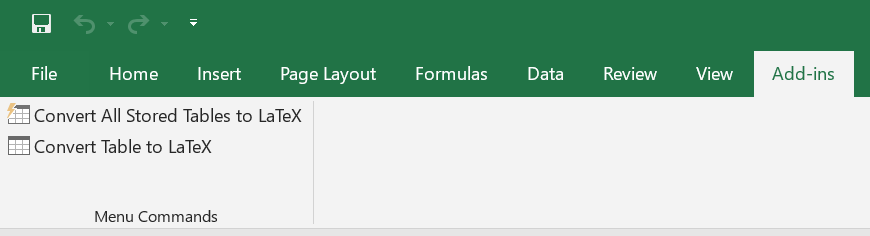
\includegraphics[width=0.6\textwidth]{excel2latex.png}
\caption{Excel2\LaTeX{} 插件\label{fig:excel2latex}}
\end{figure}


另外在线转换的工具 \href{https://tableconvert.com/?output=latex}{Table Convert} 也可以尝试一下。


\subsection{回归表格}

outreg2

R

Python

\section{颜色}

在 \LaTeX{} 中,有 7 种内置的颜色,分别是 white, black, red, green, blue, cyan, magenta, yellow。

\subsection{定义颜色}

\subsection{使用颜色}




\section{文献}

\subsection{thebibliography 环境}

\subsection{\hologo{BibTeX} 的使用}

\subsection{natbib 包}

\section{幻灯片}
Beamer 是 \LaTeX{} 用于制作幻灯片的一个文类,由于它的格式简洁、易于使用、方便展示数学公式和逻辑演绎,在学术界特别是国外非常受欢迎。下面分别是是英文 Beamer 和中文 Beamer 的一个简单示例:

\begin{code}
\documentclass{beamer}

% title information
\title{An Example of Beamer Class}
\author{Dongsheng DENG}
\institute{Fudan University}
\date{\today}

\begin{document}
\maketitle

\begin{frame}{frame title}
Be honest rather clever.
\end{frame}

\end{document}
\end{code}
\begin{rcode}
\documentclass{beamer}
\usepackage[UTF8,scheme=plain]{ctex}
% 标题信息
\title{Beamer 文类示例}
\author{邓东升}
\institute{复旦大学}
\date{2019 年 10 月 23 日}

\begin{document}
\maketitle

\begin{frame}{帧标题}
有志者事竟成,百二秦关终属楚。
\end{frame}

\end{document}
\end{rcode}

\section{文档说明}

本文档使用了 \texmint{fontspec} 和  \texmint{xeCJK} 设置英文字体和中文字体,用户需要的字体列表如下:
\begin{table}[htbp]
  \centering
  \caption{本文档字体设置}
    \begin{tabular}{lccc}
    \toprule
          & \textbf{衬线字体}  & \textbf{非衬线字体} & \textbf{等宽字体}   \\
    \midrule
    英文/\texmint{fontspec}    & Amiri & \textsf{Roboto} & \texttt{Ubuntu Mono} \\
    中文/\texmint{xeCJK}   & 方正书宋简体 & \textsf{方正楷体简体} & \texttt{方正仿宋简体}  \\
    \bottomrule
    \end{tabular}%
  \label{tab:fontset}%
\end{table}%

需要注意的是,在 Win 10 中,安装字体时需要\textsf{\textcolor{FireBrick}{为所有用户安装}},否则即便安装了字体,\LaTeX{} 也无法找到。

另外,本文高亮使用了 \texmint{minted} 宏包,所以,需要调用 \mintinline{shell}{-shell-escape} 选项并用 \hologo{XeLaTeX} 进行编译,如果使用命令行编译,命令如下:
\begin{minted}{shell}
xelatex --shell-escape main.tex
\end{minted}


\section{代码写作风格}
越来越觉得,形成固定的代码风格非常重要,包括文件命名规则。

\bibliographystyle{plainnat}
\nocite{overleaftables,overleafbibtex}
\bibliography{reference}

\end{document}
